\subsection*{Commitment Schemes}

Using hash functions, we can build secure \emph{commitment schemes}\index{Commitment Scheme}.
A commitment scheme involves a \emph{sender} and a \emph{receiver}. The sender initially
\emph{commits} to a value and sends the commitment to the receiver. At a later time, the
sender reveals the original value, and the receiver can check this. The commitment scheme
is secure if the receiver cannot ascertain the value before the revelation, and the sender
cannot change the value after the commitment. Let us make these requirements a bit more
formal through the use of cryptographic games.
The commitment scheme consists of one algorithm called \textsf{Commit} (ran by the sender)
and one algorithm called \textsf{Check} (ran by the receiver).
The \textsf{Commit} function accepts a value $v$ and returns a commitment $h$ and a randomness
$r$ which can be used at a later time. The sender initially invokes the \textsf{Commit}
function with the value $v$ and obtains $h$ and $r$. He then sends $h$ to the receiver.
When the sender is ready to reveal the value, he sends both $v$ and $r$ to the receiver.
The receiver uses the \textsf{Check} function to check the consistency of the reveal.
The \textsf{Check} function accepts a commitment $h$, a value $v$,
and the randomness $r$ and returns \textsf{true} if the reveal is consistent with the
commitment, or \textsf{false} otherwise.

We need our commitment
scheme to be \emph{correct}: If \emph{both} the verifier and prover are honest, the \emph{Verify}
function should output \emph{true}. This is captured in the following definition:

\begin{definition}[Commitment Correctness]
  A commitment scheme $(\textsf{Commit}, \textsf{Check})$ is \emph{correct} if
  for all $v$:
  $(h, r) \gets \textsf{Commit}(v); \textsf{Check}(h, v, r) = \true$.
\end{definition}

For the \emph{correctness} part, we are not speaking of negligibility or probabilities
or adversaries at all. The scheme must \emph{always} work between honest parties.

Let us now state our goals for
a secure commitment scheme in the form of a game.
We want the commitment scheme to be
\emph{binding} and \emph{hiding}. The \emph{binding} property means that the sender
cannot change his mind at a later time. Once a commitment is sent to the receiver,
only one value can be later revealed and correctly verified by the receiver. The
binding property protects the honest receiver from a malicious sender. On the
other hand, the \emph{hiding} property means that the receiver cannot deduce
any information about the sender's value prior to the time of the reveal phase.
The hiding property protects the honest sender from a malicious sender.

\import{./}{algorithms/alg.commit-game}

The games describing these security properties of the commitment scheme are
illustrated in Algorithm~\ref{alg.commit-game}. Let us look at these games a bit
more closely. In the \emph{binding-game}, we have the adversary output \emph{one}
commitment $h$, but multiple reveals $v_1$ and $v_2$ with potentially different
randomnesses $r_1$ and $r_2$. The two reveals $v_1$ and $v_2$ must be different.
The challenger then checks that both the values $v_1$ and $v_2$ verify with
the commitment $h$ using their respective randomnesses $r_1$ and $r_2$. If both
do, then the adversary was successful in breaking the binding property. Note here
that the adversary didn't have to use the honest \emph{Commit} method at all.
She was allowed to generate the values in any way she pleased. Since the \emph{binding}
property is about protecting the honest \emph{receiver}, the challenger game only uses
the honest \emph{Check} method.

On the other hand, the \emph{hiding-game} invokes the adversary twice. In the first
invocation, the adversary is asked to output two values $v_1$ and $v_2$ (for the
adversary's sake, these better be different). The challenger then flips a coin $b$
to decide between one of these two values $v_1$ or $v_2$. He then uses \emph{Commit}
to commit to the chosen value, and asks the adversary, through a second invocation,
whether she can guess which value he committed to. If the adversary can guess between
the two, she was successful in breaking the \emph{hiding} property. Again, the adversary
can use any method she pleases and is not required to invoke the \emph{Check} function
at all. In this game, since we are protecting the honest \emph{sender}, the challenger
game only uses the honest \emph{Commit} method. Additionally, observe how much power
we give to the adversary: She is completely free to choose $v_1$ and $v_2$ and they
are not chosen randomly. In case she is able to distinguish between \emph{any} such
commitments of her choice, the hiding property breaks. Our scheme will be quite
secure if we can achieve this property!

Given these properties, the security definition for commitment schemes is straightforward:

\begin{definition}[Secure Commitment Scheme]
  A commitment scheme (\emph{Commit}, \emph{Check}) is secure if there exists a
  negligible function \emph{negl} such that:

  \begin{gather*}
    \forall PPT \mathcal{A}:\\
    \textsf{binding-game}_{\emph{Commit},\emph{Check},\mathcal{A}}(\kappa) < \textsf{negl}(\kappa)\\
    \land\\
    \textsf{hiding-game}_{\emph{Commit},\emph{Check},\mathcal{A}}(\kappa) < \frac{1}{2} + \textsf{negl}(\kappa)\\
  \end{gather*}
\end{definition}

Notice here how we require that the adversary wins with only negligible probability in the \emph{binding game},
but with probability bounded by $\frac{1}{2} + \textsf{negl}$ in the \emph{hiding game}. In the hiding game,
the adversary can always succeed with probability $\frac{1}{2}$ by taking a simple random guess. This is fine.
What the security definition is saying is that the adversary cannot take any \emph{educated} guesses.

\subsection*{Commitment through Hashing}

It should now be pretty clear that we can use hash functions to create a commitment scheme. See if you can
sketch down the construction yourself before you read further. It is illustrated in Algorithm~\ref{alg.hash-commit}.
For committing, the construction generates a fresh new randomness and then applies the hash function
on the randomness and the value to be committed concatenated. This randomness is known as a \emph{salt}\index{Salt}
and is necessary for the security of the scheme (see Problem~\ref{prob.commit-salt}). The \emph{Check} function
simply applies the same hash function again to ensure that the commitment took place correctly.

\import{./}{algorithms/alg.hash-commit}

The fact that this construction is \emph{correct} should be obvious because the \emph{Commit} and
\emph{Check} algorithms both use the hash function identically.
Let us prove that this construction has the \emph{binding} property.

\import{./}{algorithms/alg.commit-security}

\begin{figure}[h]
    \centering
    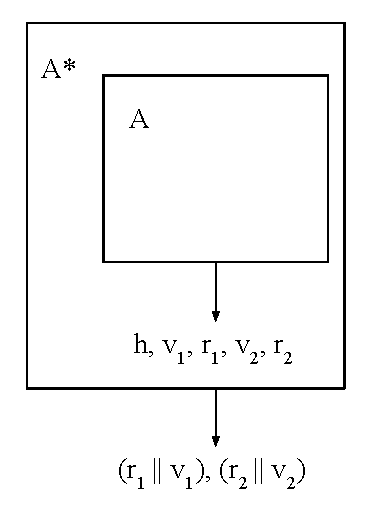
\includegraphics[width=0.35 \columnwidth,keepaspectratio]{figures/hash-commitment-reduction.pdf}
    \caption{The adversary $\mathcal{A}^*$ contains the code of $\mathcal{A}$ inside her. The outside
             adversary invokes the inside adversary to obtain the data that she later uses in her own
             response to her own challenger.}
    \label{fig.hash-commitment-reduction}
\end{figure}

\begin{theorem}[Commitment Security]
  The commitment scheme of Algorithm~\ref{alg.hash-commit} constructed using a \emph{secure
  hash function} $H$ is \emph{binding}.
\end{theorem}
\begin{proof}
  Consider any \emph{arbitrary}
  PPT adversary $\mathcal{A}$ that attempts to break the \emph{binding} property of the commitment scheme.
  We will prove that this adversary has only a negligible probability of success.
  We will construct a different adversary, $\mathcal{A}^*$, that attempts to break the \emph{collision resistance}
  property of $H$.

  The adversary $\mathcal{A}^*$ is depicted in \ref{alg.commit-security} and illustrated in
  Figure~\ref{fig.hash-commitment-reduction}. Let us observe some facts about these adversaries. First,
  the adversary $\mathcal{A}^*$ can make use of the adversary $\mathcal{A}$, because $\mathcal{A}^*$
  can simply have the code of $\mathcal{A}$ copy/pasted inside her own algorithm. Secondly,
  the adversary $\mathcal{A}^*$ is polynomial as long as $\mathcal{A}$ is polynomial, because
  $\mathcal{A}^*$ only executes a constant number of extra instructions in addition to invoking
  $\mathcal{A}$. Therefore, $\mathcal{A}^*$ is also a PPT algorithm. Lastly, these two adversaries
  will have different challengers: $\mathcal{A}$ is designed to succeed in the \emph{collision-game}
  challenger, while $\mathcal{A}^*$ is designed to succeed in the \emph{binding-game} challenger.
  One more thing to note is that we made this reduction without knowing anything about the
  nature of $\mathcal{A}$ beyond the fact that it is a PPT. Its code could be anything.

  Now for the probabilities of success, it is possible that $\mathcal{A}$ succeeds or fails.
  If $\mathcal{A}$ fails, we have no expectations of $\mathcal{A}^*$. But if $\mathcal{A}$ succeeds,
  then $\mathcal{A}^*$ always succeeds, too. The reason is the check performed by the \emph{binding-game}
  ensure that $\textsf{Verify}(h, v_1, r_1)$ and $\textsf{Verify}(h, v_2, r_2)$, but $v_1 \neq v_2$.
  But this means that $H(r_1 \conc v_1) = h$ and $H(r_2 \conc v_2) = h$, therefore
  $H(r_1 \conc v_1) = H(r_2 \conc v_2)$. But $r_1 \conc v_1 \neq r_2 \conc v_2$. To see this,
  note that $r_1$ and $r_2$ have the same length and could be equal, but $v_1$ and $v_2$ are different.
  Therefore, the check performed by the \emph{collision-game} will succeed.

  We conclude that, if $\mathcal{A}$ succeeds, then $\mathcal{A}^*$ succeeds, and s
  the probability of success of $\mathcal{A}^*$ against the \emph{collision-game}
  is at least as much as the probability of of success $\mathcal{A}$ against the \emph{binding-game}
  (in fact the two probabilities happen to be equal):

  \[
    \Pr[\textsf{collision-game}_{H,\mathcal{A}^*}(1^\kappa)] \geq
    \Pr[\textsf{binding-game}_{\textsf{Commit},\textsf{Check},\mathcal{A}}(1^\kappa)]
  \]

  From the assumption that $H$ is collision resistant, we know that

  \[
    \Pr[\textsf{collision-game}_{H,\mathcal{A}^*}(1^\kappa)] < \textsf{negl}\,.
  \]

  Therefore, applying the above inequality,
  $\Pr[\textsf{binding-game}_{\textsf{Commit},\textsf{Check},\mathcal{A}}(1^\kappa)] < \textsf{negl}$,
  too.
\end{proof}

This proof is a standard reduction proof that follows the outline we gave in Chapter~\ref{chapter.untrusty-world}.
Note how we skipped the $\kappa$ as a parameter to the \emph{negl} function, since it is clear
from context.

We proved that \emph{binding} follows from \emph{collision resistance}. It would seem that
\emph{hiding} must follow from \emph{preimage resistance}, but, even though this scheme is
hiding in practice, the proof will require a different model (see Problem~\ref{prob.preimage-no-hide}).

\section*{Problems}

\begin{enumerate}
  \item Consider a hash-based commitment scheme construction in which no salt is used.
        Prove that the scheme is correct. Use collision resistance to prove that the scheme is binding.
        Calculate the probability of success of a hiding adversary in the
        hiding game.\label{prob.commit-salt}
  \item Construct a correct commitment scheme which is hiding but not binding.
  \item Construct a correct commitment scheme which is binding but not hiding.
  \item Show that the hash-based commitment scheme constructed using a
        pathological secure hash function may not be hiding.
        (Hint: Start with a secure hash function $H$ and modify it
         to obtain a pathological secure hash function $H^*$.)\label{prob.preimage-no-hide}
\end{enumerate}